\section{Next-to-leading order and renormalization}
We have now regularized the divergences, so they can be handled in a well-defined way.
However, they are still there.
To get rid of them, we need to use renormalization.
The power counting scheme used when constructing the Effective Lagrangians ensures that all terms in $\Ell_{2n}$ is of order $p^{2n}$ in the pion momenta.\footnote{Remember that the pion mass $m_\pi = 2 f_\pi B$ is considered to be of order $p^2$.}
The tree level free energy from $\Ell_{2n}$ is thus of order $p^{2n}$.
The n-loop correction to the tree level result is then suppressed by $p^{2n}$~\cite{Gasser-Leutwyler:chiral,WeinbergPhenom}.
Our one-loop calculation using $\Ell_2$ therefore contains divergences of order $p^{4}$. 
Since $\Ell_4$ is, by construction, the most general possible Lagrangian at order $p^4$, it contains coupling constants which can be renormalized to absorb all these divergences.

The renormalized coupling constants in $\Ell_2$ have been calculated for $\mu_I = 0$~\cite{Gasser-Leutwyler:chiral}.
They are independent of $\mu_I$, and we can therefore use them in this calculation.
The renormalized coupling constants in the $\overline{\mathrm{MS}}$-scheme are related to the bare couplings through
\begin{align}
    l_i 
    & = 
    l_i^r \, \,
    - \frac{1}{2} \frac{\gamma_i }{(4 \pi)^2} 
    \left(\frac{1}{\epsilon} + 1 - \ln \mu^2\right),
    \quad \quad
    i \in \{1, ... 7\} 
    \\
    h_i 
    & = 
    h_i^r
    - \frac{1}{2} \frac{\delta_i }{(4 \pi)^2} 
    \left(\frac{1}{\epsilon} + 1 - \ln \mu^2 \right), 
    \quad \quad
    i \in \{1, ... 3\}.
\end{align}
(HVORDAN KAN VI HA log AV DIMENSJONSFULL STØRRELSE?).
Here, $\gamma_i$ and $\delta_i$ are numerical constants that are used to match the divergences.
The relevant terms are
\begin{gather}
    \gamma_1 = \frac{1}{3}, \quad
    \gamma_2 = \frac{2}{3}, \quad
    \gamma_3 = - \frac{1}{2}, \quad
    \gamma_4 = 2, \\
    \delta_1 = 2, \quad
    \delta_3 = 0.
\end{gather}
The bare coupling constants, though infinite, are independent of our renormalization scale $\mu$.
From this we obtain the renormalization group equations for the running coupling constants,
\begin{equation}
    \diff{\, l_i^r}{\ln \mu } = - \frac{\gamma_i}{(4 \pi)^2}, \quad
    \diff{\, h_i^r}{\ln \mu } = - \frac{\delta_i}{(4 \pi)^2}.
\end{equation}
These have the general solutions
\begin{equation}
    l_i^r 
    = \frac{1}{2} \frac{\gamma_i}{(2 \pi)^2} 
    \left( \bar l_i - \ln{\frac{\mu^2}{M^2}} \right),
    \quad
    h_i^r 
    = \frac{1}{2} \frac{\gamma_i}{(2 \pi)^2} 
    \left( \bar h_i - \ln{\frac{\mu^2}{M^2}} \right),
\end{equation}
where $\bar l_i$ and $\bar h_i$ are the values of the coupling constants (times a constant) measured at the energy $M$.
This only applies if the numerical constants $\gamma_i$/$\delta_i$ are non-zero.
If they are zero, then the renormalized constant is not running, and instead equal to its measured value at all energies.
The bare couplings are thus given by
\begin{equation}
    l_i = \frac{1}{2} \frac{\gamma_i}{(4 \pi)^2}
    \left(\bar l_i - 1 - \frac{1}{\epsilon} - \ln\frac{\mu^2}{M^2}\right), \quad
    h_i = \frac{1}{2} \frac{\delta_i}{(4 \pi)^2}
    \left(\bar h_i - 1 - \frac{1}{\epsilon} - \ln\frac{\mu^2}{M^2}\right)
\end{equation}
(HVOR BLE DET AV $\ln \mu$?)
The free energy at tree-level, at next-to-leading order is, according to \cref{NLO-L0}, 
\begin{align*}
    \Ef^{(0)}_4
    & 
    = - \Ell_4^{(0)} 
    \\
    & = 
    - (l_1 + l_2)\mu_I^4 \sin^4{\alpha}
    - (l_3 + l_4)(2 B_0 \bar m)^2 \cos^2{\alpha}
    - l_4 (2 B_0 \bar m ) \mu_I{}^2 \cos{\alpha} \sin^2{\alpha}
    \\
    & 
    \quad -(h_1- l_4) (2B_0 \bar m )^2
    - h_3 (2B_0 \Delta m)^2
    % \\
    % & = 
    % - \frac{1}{2} \frac{1}{(4 \pi)^2}
    % \bigg[
    %     \frac{1}{3}
    %     \left( 
    %         \bar l_1 + 2 \bar l_2 - 3 - \frac{3}{\epsilon} - 3\ln \frac{\mu^2}{M^2}
    %     \right) \mu_I^4 \sin^4 \alpha
    %     +
    %     \frac{1}{2}
    %     \left(
    %         - \bar l_3 + 4 \bar l_4 - 3 - \frac{3}{\epsilon} - 3\ln \frac{\mu^2}{M^2}
    %     \right) (2 B_0 m)^4 \cos^2\alpha 
    %     \\
    %     &
    %     + 2 \left(\bar l_4 - 1 - \frac{1}{\epsilon} - \ln \frac{\mu^2}{M^2} \right)
    %     (2 B_0 m)^2 \mu_I^2 \cos\alpha \sin^2 \alpha
    %     + 2 (\bar l_4 - \bar h_1) (2B_0 \bar m )^2
    %     + \bar h_3 (2B_0 \Delta m)^2    
    % \bigg]
    \\
    & = 
    - \frac{1}{2} \frac{1}{(4 \pi)^2}
    \bigg[
        \frac{1}{3}
        \left( 
            \bar l_1 + 2 \bar l_2 - 3
        \right) \mu_I^4 \sin^4 \alpha
        +
        \frac{1}{2}
        \left(
            - \bar l_3 + 4 \bar l_4 - 3
        \right) (2 B_0 m)^4 \cos^2\alpha
        \\
        & \quad \quad \quad \quad \quad
        + 2 \left(\bar l_4 - 1\right)
        (2 B_0 m)^2 \mu_I^2 \cos\alpha \sin^2 \alpha
        + 2 (\bar l_4 - \bar h_1) (2B_0 \bar m )^2
        + \bar h_3 (2B_0 \Delta m)^2
        \\
        & \quad \quad \quad \quad \quad
        - 
        \left(\frac{1}{\epsilon} + \ln \frac{\mu^2}{M^2}\right) 
        \left(
            \mu_I^4\sin^4\alpha + \frac{3}{2} (2 B_0 m)^4 \cos^2 \alpha
            + 2 (2 B_0 m)^2 \mu_I^2 \cos\alpha \sin^2 \alpha
        \right) 
        % \\
        % & \quad \quad \quad \quad \quad
    \bigg] 
\end{align*}
Adding all the contribution to the free energy density, we get the next-to-leading order free energy,
\begin{align}
    \nonumber
    \Ef_{\mathrm{NLO}} &=
    - f^2 \left((2 B_0 m)^2 \cos \alpha + \frac{1}{2}\mu_I^2 \sin^2 \alpha\right)
    + \Ef^{(1)}_{\mathrm{fin}, \pi_\pm}
    - \frac{1}{2}\frac{1}{(4 \pi)^2}
    \bigg[
        \frac{1}{3}
        \left( 
            \bar l_1 + 2 \bar l_2 + \frac{3}{2} + 3 \ln \frac{M^2}{m_3^2}
        \right) \mu_I^4 \sin^4 \alpha
        \\ \nonumber
        &
        +
        \frac{1}{2}
        \left(
            - \bar l_3 + 4 \bar l_4 + \frac{3}{2} + 2\ln \frac{M^2}{m_3^2}
            + \ln \frac{M^2}{\tilde m^2_2}
        \right) (2 B_0 m)^4 \cos^2\alpha 
        + 2 \left(\bar l_4 - \frac{1}{2} + \ln \frac{M^2}{m_3^2}\right)
        (2 B_0 m)^2 \mu_I^2 \cos\alpha \sin^2 \alpha
        \\ \label{NLO free energy}
        & 
        + 2 (\bar l_4 - \bar h_1) (2B_0 \bar m )^2
        + \bar h_3 (2B_0 \Delta m)^2
    \bigg].
\end{align}
The next-to-leading order result for $\alpha$ as a function of $\mu_I$ is given by 
\begin{eqnarray}
    \diff{\Ef}{\alpha} = 0,
\end{eqnarray}
using the result \cref{NLO free energy}.
In \autoref{fig:alpha}, the NLO result is compared with the LO result, \cref{leading order minization}.

\begin{figure}
    \centering
    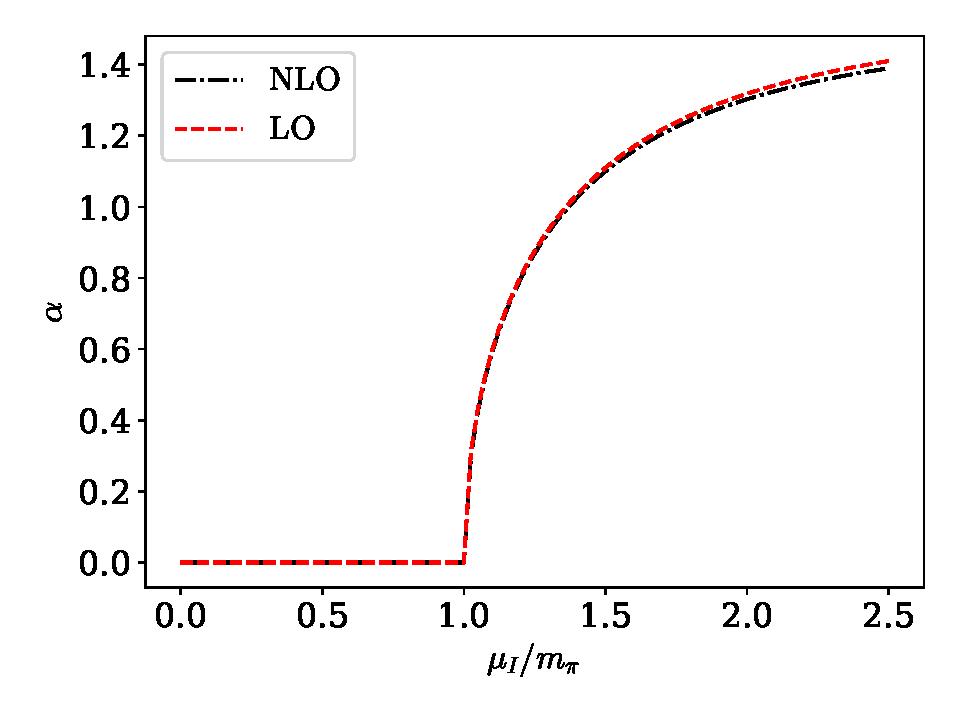
\includegraphics[width=0.7\textwidth]{figurer/numerics/alpha.pdf}
    \caption{The leading order and next-to-leading order results for $\alpha$ as a function of $\mu_I$.}
    \label{fig:alpha}
\end{figure}

